\chapter{Introduction}
\label{sec:intro} 

Internet censorship is a significant and growing problem that threatens our freedom of expression and access to information. A citizen within a censored country attempts to access the internet that is hosted beyond the censor's control boundary, shown in Figure \ref{fig:simplecensor}. A censor is a strong nation state adversary that conducts mass surveillance and utilizes blacklists. One of the simplest techniques employed by censors is to deny access to users by blocking traffic destined for blacklisted sites. 

%%%%%%%%%%%%%%%%%%%%%%%%%%%%%%%%%%%%%%%%%%%%%%%%%%%%%%%%%%%%%%%%%%%%%%
\begin{figure*}[h!]
\centering
     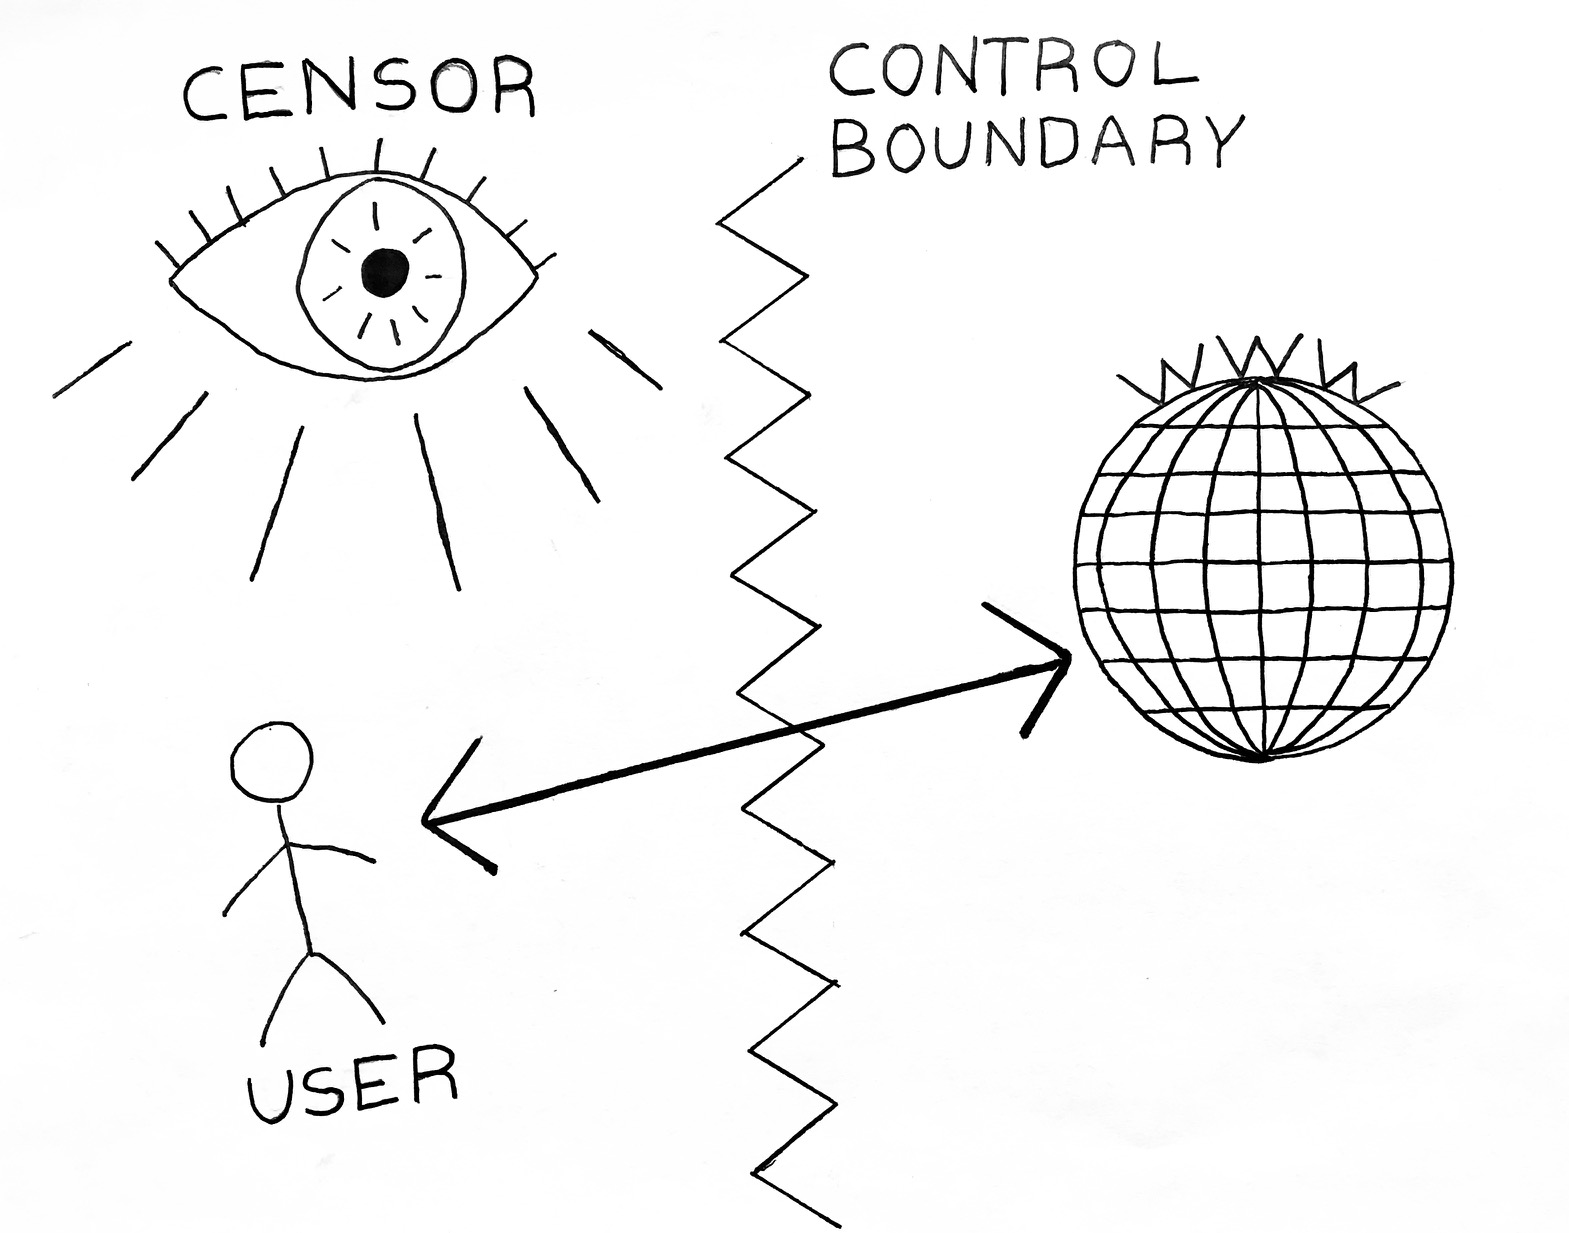
\includegraphics[width=0.5\textwidth]{fig/censor_simple_new.png}
    \caption{A censor observes a citizen's network activity.}
    
    \label{fig:simplecensor}
\end{figure*}
%%%%%%%%%%%%%%%%%%%%%%%%%%%%%%%%%%%%%%%%%%%%%%%%%%%%%%%%%%%%%%%%%%%%%%

This effective censorship technique can be circumvented by means of proxies; single-hop servers outside of the censored country that facilitate indirect access to censored information. In Figure \ref{fig:censorblock}, a citizen is blocked from the internet but manages to access sites via a proxy. \ac{CRS} like rBridge \cite{wang2013rbridge}, meek \cite{Fifield2017a}, and Tor's \texttt{bridgedb} \cite{BridgeDB:2019} manage proxies and allow users in censored countries to access blacklisted websites. These systems bypass censors and route users through secret paths. Secret paths rely on proxies that are managed by censorship resistance systems. Proxies serve as intermediary hops between a user and a blacklisted destination site.

%%%%%%%%%%%%%%%%%%%%%%%%%%%%%%%%%%%%%%%%%%%%%%%%%%%%%%%%%%%%%%%%%%%%%%
\begin{figure*}[h!]
\centering
     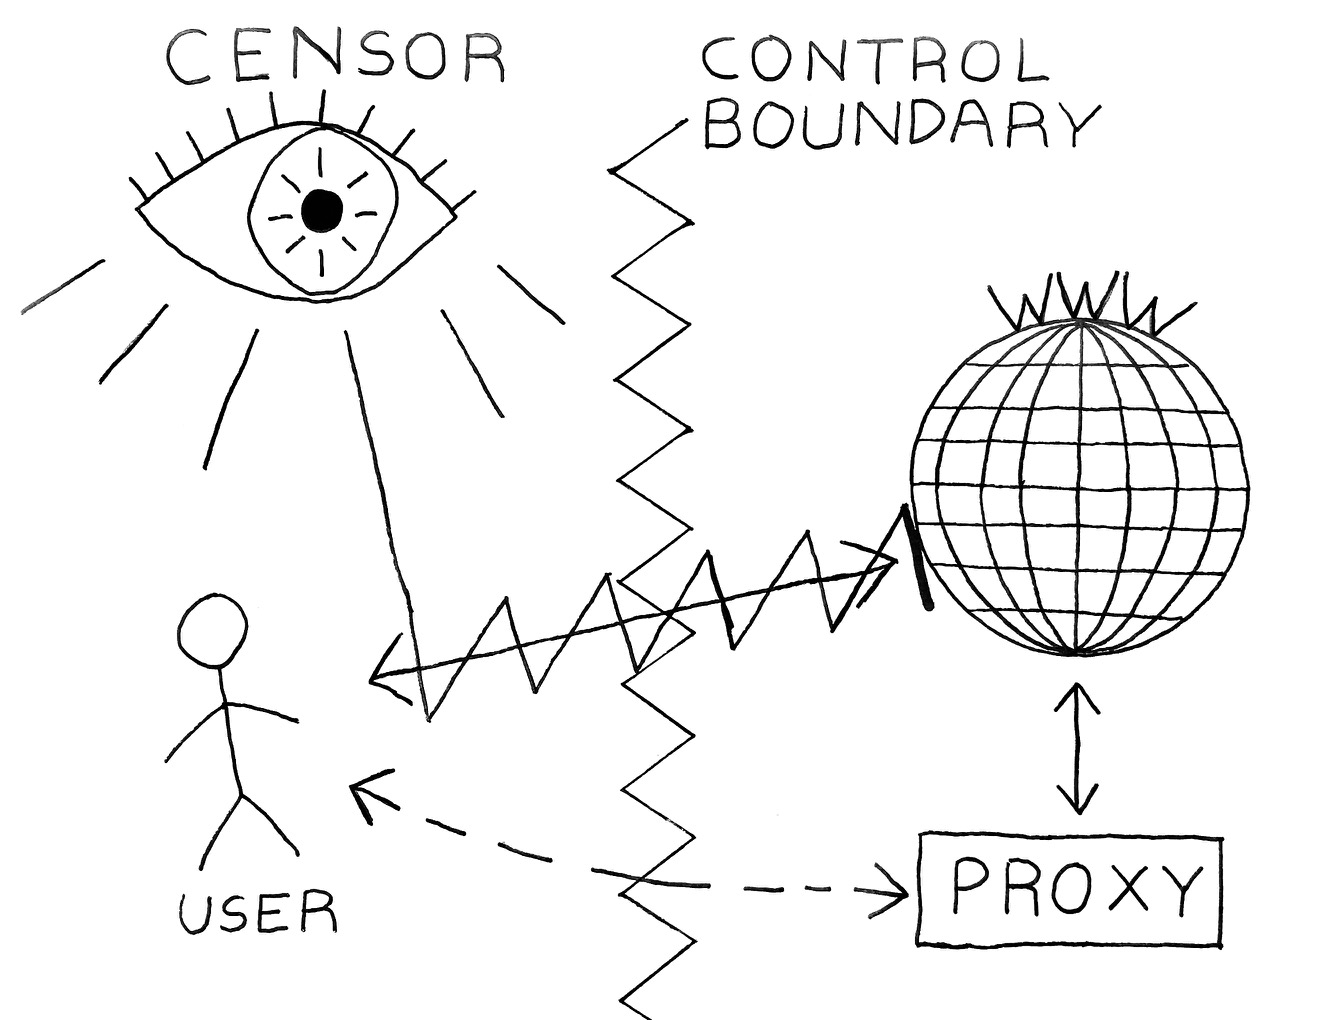
\includegraphics[width=0.6\textwidth]{fig/censor_block_new1.png}
    \caption{The citizen uses a proxy to access the internet.}
    
    \label{fig:censorblock}
\end{figure*}
%%%%%%%%%%%%%%%%%%%%%%%%%%%%%%%%%%%%%%%%%%%%%%%%%%%%%%%%%%%%%%%%%%%%%%

\ac{CRS} are composed of honest and dishonest (fake) users, several honest proxies, and a centralized proxy distributor that is also honest. Figure \ref{fig:proxydistro} shows a typical censorship circumvention system using a collection of proxies and a centralized distributor. \ac{CRS} rely on the proxy distributor to assign clients to proxies. Honest users anonymously request proxies and receive proxy information details from the distributor. However, a censor may also learn proxy details by posing as an honest user via legitimate, anonymous methods. The censor coordinates information collected through a collection of fake accounts to gain knowledge of the proxies in the circumvention system.

%%%%%%%%%%%%%%%%%%%%%%%%%%%%%%%%%%%%%%%%%%%%%%%%%%%%%%%%%%%%%%%%%%%%%%
\begin{figure*}[h!]
\centering
     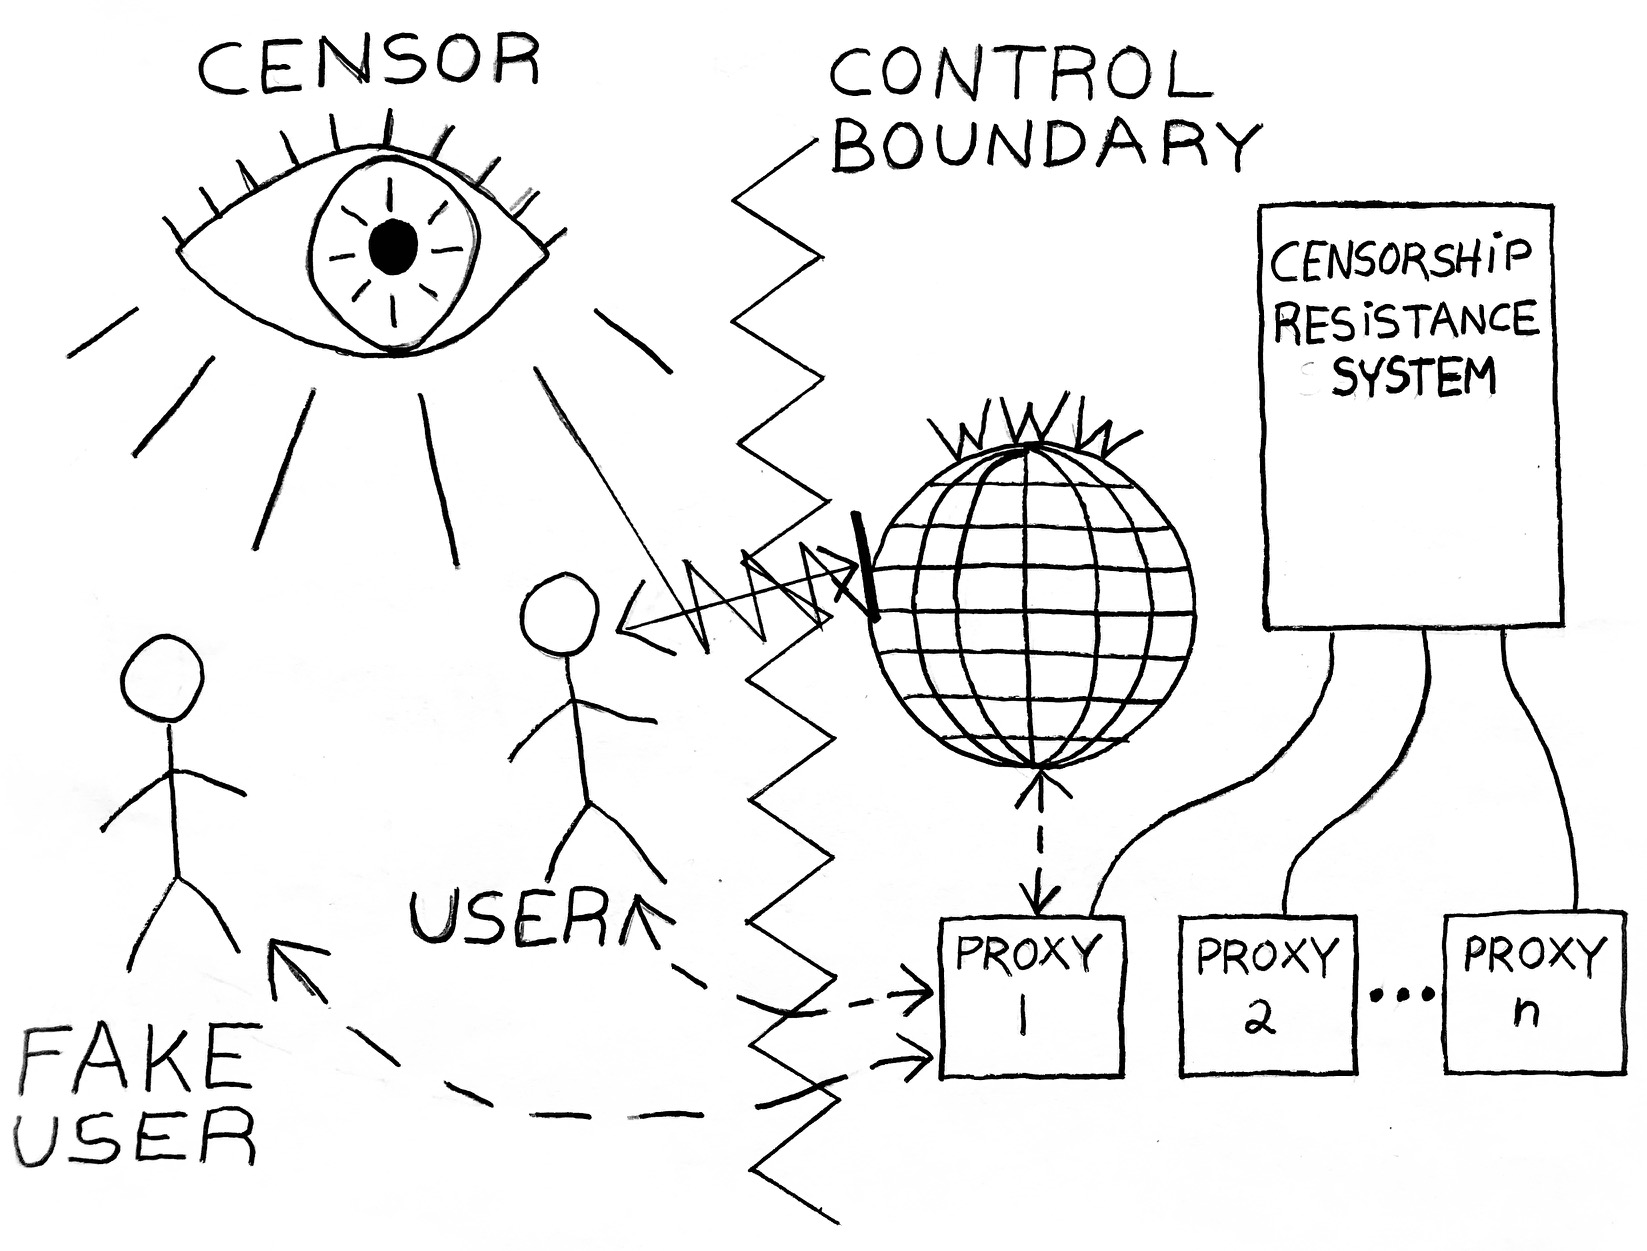
\includegraphics[width=0.6\textwidth]{fig/censor_crs_new.png}
    \caption{Censorship circumvention via proxy distribution.}
    \label{fig:proxydistro}
\end{figure*}
%%%%%%%%%%%%%%%%%%%%%%%%%%%%%%%%%%%%%%%%%%%%%%%%%%%%%%%%%%%%%%%%%%%%%

To get an idea of the scale of censorship events around the world, Figure \ref{fig:oonimap} shows a world map where the \ac{OONI} project's network measurement tests, \texttt{ooniprobes}, are run daily by volunteers \cite{OONI:2019}. The red areas on the map outline confirmed cases of censorship. Censorship is confirmed by the response body of a \ac{HTTP} request of a blocked page from within a censored country.

%%%%%%%%%%%%%%%%%%%%%%%%%%%%%%%%%%%%%%%%%%%%%%%%%%%%%%%%%%%%%%%%%%%%%%
\begin{figure*}[h!]
\centering
     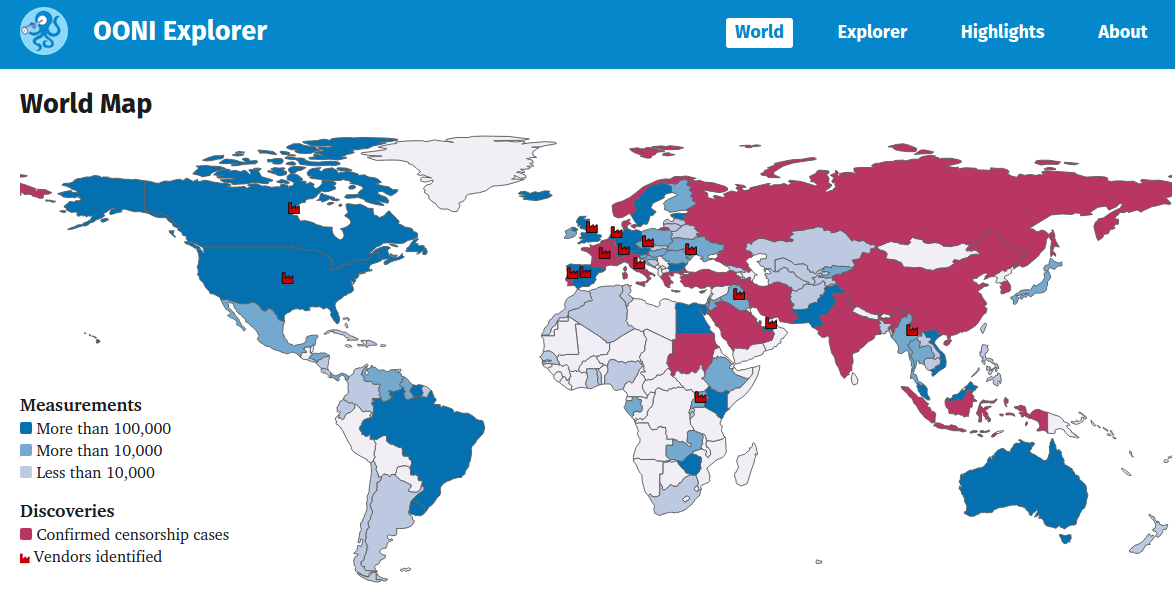
\includegraphics[width=1.0\textwidth]{fig/ooni_map.png}
    \caption{\ac{OONI} project's censorship data.}
    
    \label{fig:oonimap}
\end{figure*}
%%%%%%%%%%%%%%%%%%%%%%%%%%%%%%%%%%%%%%%%%%%%%%%%%%%%%%%%%%%%%%%%%%%%%%

Proxies in censorship resistance systems that cannot distinguish between honest users and fake users are destined for discovery over time. Most systems manually \textit{reserve} a set of proxies that is only distributed when all other proxies are compromised. This manual solution is effective, but does not maximize the allocation of proxies. 

We offer a lightweight, elegant solution to the proxy distribution problem by slowing down the progress of the censor to learn new proxies. Our goal is to provide service to clients while \textit{preserving} proxies from distribution, a goal that is complimentary to \textit{reserving} proxies. We introduce a partially random strategy for the proxy distribution problem to distribute proxies to honest clients while fake clients are present. Our approach uses principles of load balancing in a non-intuitive way to preserve random proxies by unbalancing the load on proxies, making them more difficult to discover. 

We provide an approximation of the censor's required effort to discover all of the proxies in a system based on the coupon collector problem \cite{flajolet1992birthday}. We validate this approach in a simulator that simulates a proxy distributor in a censorship resistance system. \\

We contribute to the existing body of knowledge in the following five ways:
\begin{enumerate}
    \item We introduce a novel algorithm, \emph{needle}, that restricts the distribution of proxies in order to slow the expected time of proxy system compromise while still maintaining service to a proportion of clients.
    \item We define a censorship threat model within which we evaluate the needle algorithm. We define honest users, a proxy distributor, insider attackers, popularity blocking, and a colluding censor within this model.
    \item We analyze the needle algorithm in the context of the coupon collector problem to give bounds on the average time to collect all of the proxies.
    \item We build a simulator to evaluate the needle proxy distribution algorithm and compare the results with Tor's \texttt{bridgedb} distribution, uniform random distribution, and the power of 2 choice load balancing algorithms. 
    \item We discuss the benefits and drawbacks of trust-based proxy distribution vs. lightweight approaches and provide ideas for future work on our approach.
\end{enumerate}